\documentclass[review,nopreprintline]{elsarticle}
\usepackage{lineno}
\usepackage{amssymb}
\usepackage{amsmath}
\usepackage{booktabs}
\usepackage{longtable}
\usepackage{tabularx}
\usepackage{siunitx}
\usepackage{enumitem}
\usepackage{graphicx}
\usepackage{float}
\usepackage{placeins}
\usepackage{dblfloatfix}
\usepackage{xcolor}
\usepackage{hyperref}
\newcolumntype{Y}{>{\raggedright\arraybackslash}X}
\journal{Journal of Energy Storage}
\date{}
\newcommand{\code}[1]{\path{#1}}
\newcommand{\benchfig}[2]{%
\IfFileExists{#1}{\includegraphics[width=\columnwidth]{#1}}{\fbox{\parbox{0.9\columnwidth}{#2\\\path{#1}}}}%
}
\makeatletter
\renewcommand{\topfraction}{0.85}
\renewcommand{\bottomfraction}{0.85}
\renewcommand{\textfraction}{0.15}
\renewcommand{\floatpagefraction}{0.90}
\renewcommand{\dbltopfraction}{0.85}
\renewcommand{\dblfloatpagefraction}{0.90}
\setcounter{topnumber}{2}
\setcounter{bottomnumber}{2}
\setcounter{totalnumber}{4}
\setcounter{dbltopnumber}{2}
\makeatother
\raggedbottom

\begin{document}
\begin{frontmatter}
\title{Performance Benchmarking of Embedded Battery State Estimation: A Measurement-Only Comparison of Direct-Measurement, Hybrid, and Data-Driven Estimators}
\author[1]{Florian Rzepka\corref{cor1}}
\ead{florian.rzepka@tu-berlin.de}
\author[1]{Qinnan Chen}
\ead{qinnan.chen@campus.tu-berlin.de}
\author[1]{Julia Kowal}
\ead{julia.kowal@tu-berlin.de}
\cortext[cor1]{Corresponding author.}
\affiliation[1]{organization={Technical University of Berlin, Chair of Electrical Energy Storage Technology},
            addressline={Einsteinufer 11},
            city={Berlin},
            postcode={10587},
            country={Germany}}
\begin{abstract}
This paper presents a measurement-only performance benchmark for embedded battery state estimation under realistic Battery Management System (BMS) constraints. The study isolates estimator performance rather than hardware-resource or implementation-effort evaluation and compares four embedded-ready estimators on the same Lithium Iron Phosphate (LFP) full-cell trajectory under a shared embedded constraint: a direct-measurement model (DM), a hybrid direct-measurement model with learned State-of-Health support (HDM), a hybrid equivalent-circuit model with voltage feedback (HECM), and a data-driven neural model with GRU-based SOC estimation and LSTM-based online SOH context (DD). The benchmark perturbs only measurable inputs and timing information, including ADC quantization, current bias, additive current, voltage, and temperature noise, missing samples, irregular sampling, burst dropout, voltage spikes, and initial-state mismatch, so that all disturbances remain physically interpretable and reproducible. The comparison reveals no universal winner across deployment-relevant dimensions. Under clean conditions, HDM provides the lowest baseline error with an MAE of $0.0024$, followed by HECM with $0.0090$, DD with $0.0100$, and DM with $0.0311$. Under disturbed measurements, HECM is the strongest overall robustness choice, especially in the most discriminative current-bias and voltage-noise scenarios. DD is the most stable estimator under missing samples and recovers fastest after initialization mismatch, while DM shows the expected drift sensitivity and HDM trades nominal accuracy against reduced disturbance tolerance. The benchmark therefore exposes complementary failure modes of direct-measurement, hybrid physics-based, and data-driven estimators and supports decision-oriented model selection for embedded BMS deployment.
\end{abstract}
\begin{keyword}
Battery management system \sep State of charge \sep State of health \sep Performance benchmark \sep Direct measurement \sep Equivalent circuit model \sep Data-driven estimation \sep Embedded artificial intelligence
\end{keyword}
\end{frontmatter}
\linenumbers

\section*{Nomenclature}
\small
\subsection*{Acronyms}
\begin{description}[style=multiline,leftmargin=1.7cm,font=\bfseries]
\item[BMS] Battery management system
\item[SOC] State of charge
\item[SOH] State of health
\item[DM] Direct-measurement model
\item[HDM] Hybrid direct-measurement model
\item[HECM] Hybrid equivalent-circuit model
\item[DD] Data-driven neural model
\item[ECM] Equivalent circuit model
\item[EKF] Extended Kalman filter
\item[MAE] Mean absolute error
\item[RMSE] Root-mean-square error
\item[ADC] Analog-to-digital converter
\item[CV] Constant-voltage phase
\item[OCV] Open-circuit voltage
\item[GRU] Gated recurrent unit
\item[LSTM] Long short-term memory
\item[LFP] Lithium iron phosphate
\end{description}
\medskip
\subsection*{Symbols}
\begin{description}[style=multiline,leftmargin=1.7cm,font=\bfseries]
\item[$t$] Time
\item[$I(t)$] Current signal at time $t$
\item[$U(t)$] Voltage signal at time $t$
\item[$T(t)$] Temperature signal at time $t$
\item[$\widehat{\mathrm{SOC}}(t)$] Estimated state of charge at time $t$
\item[$\widehat{\mathrm{SOH}}(t)$] Estimated state of health at time $t$
\item[$\mathrm{SOC}_{\mathrm{ref}}(t)$] Reference SOC target at time $t$
\item[$\mathrm{SOH}_{\mathrm{ref}}(t)$] Reference SOH target at time $t$
\item[$\Delta I$] Current bias or offset
\item[$\Delta U$] Voltage bias or offset
\item[$\Delta T$] Temperature bias or offset
\item[$\sigma_I$] Standard deviation of injected current noise
\item[$\sigma_U$] Standard deviation of injected voltage noise
\item[$\sigma_T$] Standard deviation of injected temperature noise
\item[$Q_c$] Online cumulative charge state used by the SOC models
\item[$C_{\mathrm{nom}}$] Nominal capacity
\item[$C_{\mathrm{eff}}$] Effective capacity used inside the estimator
\item[$U_{\max}$] Upper voltage threshold used for full-charge detection
\item[$U_{\mathrm{tol}}$] Voltage tolerance used in the full-charge condition
\item[$U_{1},U_{2}$] Polarization voltages of the first and second RC branch
\item[$\Delta\mathrm{MAE}$] Error increase relative to baseline
\end{description}
\normalsize

\section{Introduction}
\subsection{Motivation and practical relevance}
Reliable battery state estimation is a core BMS function because SOC and SOH determine safety margins, usable energy, operating limits, charge control, and degradation-aware system management in both mobile and stationary lithium-ion battery applications \cite{shrivastavaReviewTechnologicalAdvancement2023,guoSystematicReviewElectrochemical2024,yaoSmarterBatteryManagement2025b}. Practical deployment quality is not defined by clean-condition accuracy alone, because real BMS operation is exposed to sensor bias, additive noise, initialization uncertainty after restart, missing samples, irregular sampling, communication interruptions, and transient signal spikes caused by measurement-chain limitations or disturbances in the surrounding system \cite{liRobustnessSOCEstimation2015,naseriReliableWirelessBMS2025,bergerBenchmarkingBatteryManagement2024}. The relevant engineering question is therefore not only whether an estimator achieves low MAE under nominal measurements, but also whether it converges back to a reliable state after disturbed initialization and whether it remains stable under physically plausible measurement corruption.

As summarized conceptually in Figure~\ref{fig:performance_requirements}, the present benchmark treats deployment-facing performance as a three-dimensional problem consisting of nominal accuracy, convergence behavior after state inconsistency, and robustness against disturbed measurements and signal-integrity faults, embedded within broader BMS requirements such as hardware constraints and implementation effort. The present study therefore isolates the performance branch and compares representative estimator classes under identical measurement-side disturbances and a matched embedded-feasibility constraint. The benchmark shows that strong nominal accuracy does not necessarily imply strong disturbance performance and that the estimator classes respond differently to bias, missing samples, and re-initialization events.

\begin{figure*}[t]
    \centering
    \IfFileExists{figures/Schematics/BMS_Requirements.png}{\makebox[\textwidth][c]{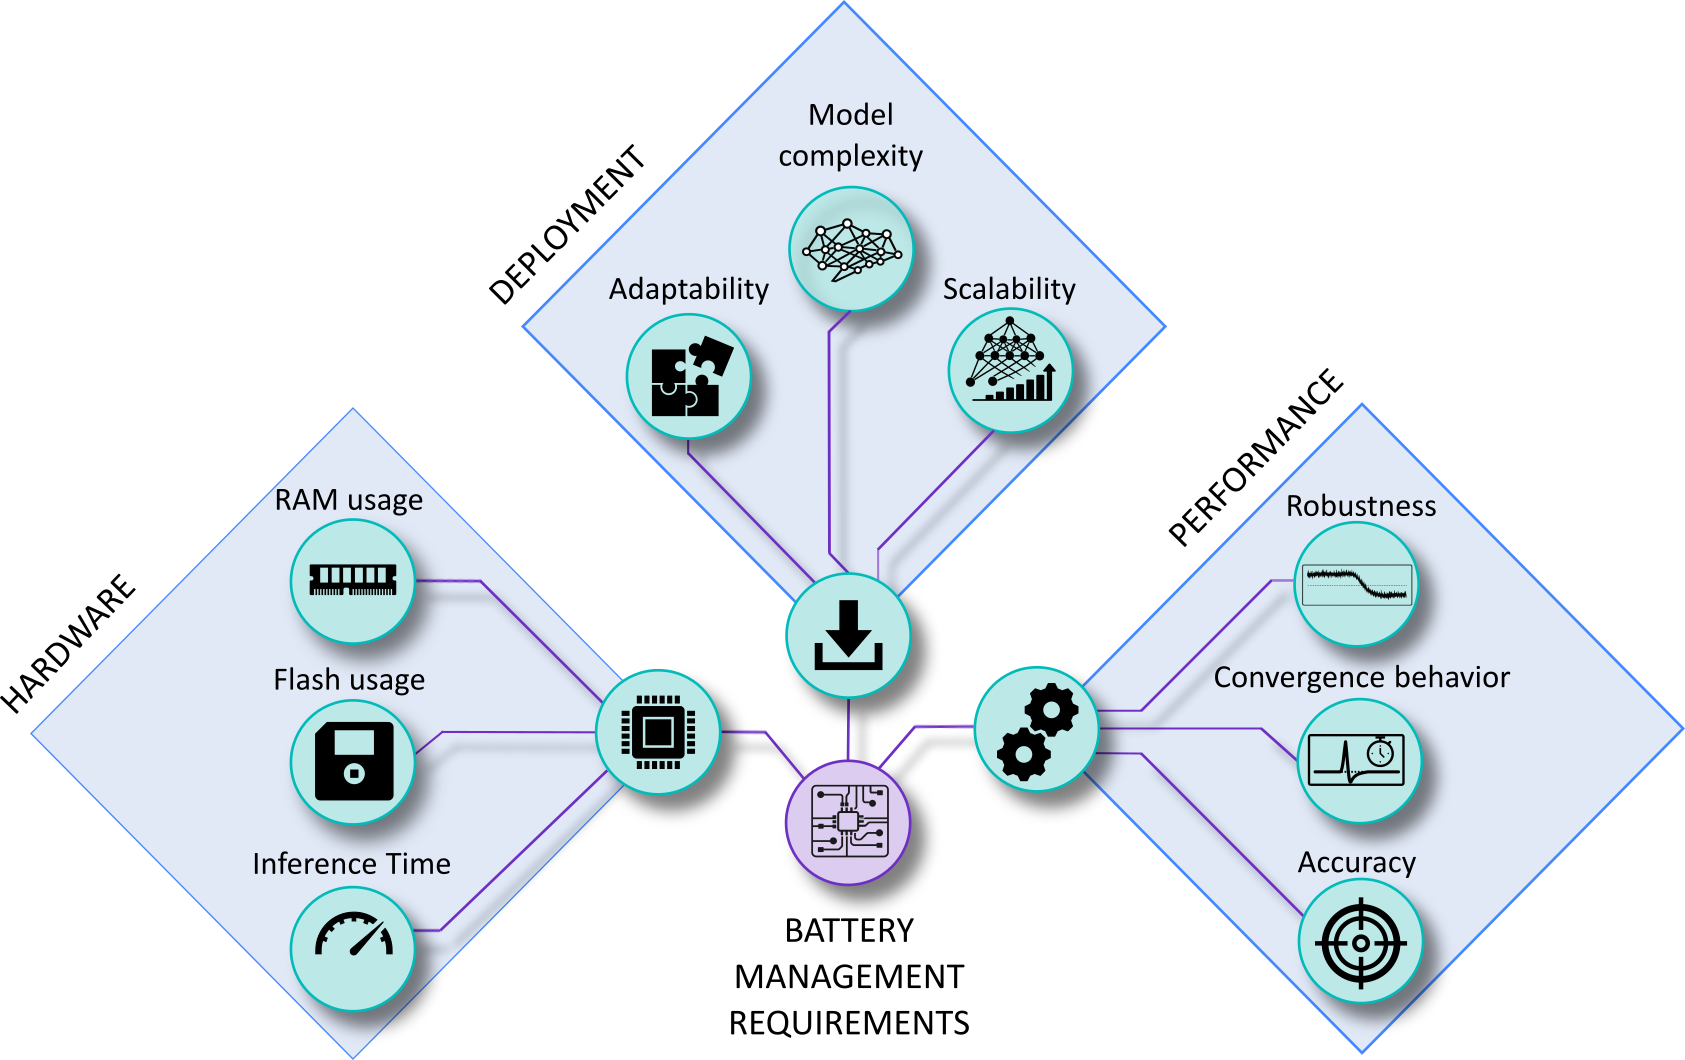
\includegraphics[width=1.04\textwidth]{figures/Schematics/BMS_Requirements.png}}}{\fbox{\parbox{0.9\textwidth}{Placeholder for an adapted conceptual overview of deployment-oriented BMS state-estimation requirements. The figure should group requirements into implementation, hardware, and performance, and should explicitly highlight that the present study focuses on the performance branch with baseline accuracy, convergence behavior, and robustness.\\\path{figures/Schematics/BMS_Requirements.png}}}}
    \caption{Conceptual overview of deployment-oriented requirements for embedded BMS state estimation. The broader requirement space includes implementation effort, hardware constraints, and estimator performance, whereas the present study focuses on the performance branch and evaluates baseline accuracy, convergence behavior, and robustness under measurement disturbances.}
    \label{fig:performance_requirements}
\end{figure*}

\subsection{State of the art in battery state estimation}
The literature commonly groups battery-state estimators into direct-measurement or integration-based approaches, model-based approaches based on equivalent-circuit or electrochemical models, hybrid approaches that combine physical structure with learned components, and purely data-driven models based on neural sequence learning \cite{khanComparativeStudyDifferent2022,shrivastavaReviewTechnologicalAdvancement2023,guoSystematicReviewElectrochemical2024,yaoSmarterBatteryManagement2025b}. Direct-measurement approaches, typically based on Coulomb counting, are attractive because they are simple, computationally inexpensive, and easy to deploy; however, they remain structurally sensitive to current bias, missing data, and initialization errors because they lack an internal correction mechanism \cite{khanComparativeStudyDifferent2022,liRobustnessSOCEstimation2015}. Model-based approaches, especially ECM- and observer-based estimators, offer physical interpretability and voltage-based correction capability, but their practical behavior depends strongly on the quality of model parametrization, operating-point observability, and measurement quality \cite{gaoEnhancedStateofchargeEstimation2022,guoSystematicReviewElectrochemical2024,liRobustnessSOCEstimation2015}.

Hybrid estimators seek to combine physical state propagation with learned adaptation of capacity, parameters, or auxiliary states, which has made joint SOC/SOH estimation an active research direction \cite{gaoCoEstimationStateofChargeStateof2022,shenAlternativeCombinedCoestimation2022,wangFusionEstimationLithiumion2022}. This combination can improve baseline calibration, while it does not necessarily eliminate structural sensitivity to measurement disturbances. Data-driven approaches based on recurrent or sequence models can exploit nonlinear cross-relations between current, voltage, temperature, and derived online features, and recent work has also demonstrated their embedded feasibility through TinyML-oriented implementations, pruning, and quantization \cite{mondalEstimatingStateofChargeLithiumIon2024,Embedded_AI_only_SOC_mobile,giazitzisCaseStudyTiny2024,mazziStateChargeEstimation2022,yaoSmarterBatteryManagement2025b}.

\subsection{Performance and embedded deployment gap}
A large share of the SOC estimation literature still emphasizes clean-data accuracy, average error metrics, or computational efficiency, while comparatively fewer studies analyze how estimators behave under realistic measurement faults and timing corruption \cite{shrivastavaReviewTechnologicalAdvancement2023,Embedded_AI_only_SOC_mobile,giazitzisCaseStudyTiny2024,mazziStateChargeEstimation2022}. Existing robustness studies often remain confined to a single model family, for example observer-based robustness against modeling and measurement errors \cite{liRobustnessSOCEstimation2015} or robust estimation concepts for specific BMS architectures under noise and uncertainty \cite{naseriReliableWirelessBMS2025}, whereas cross-family comparisons under the same disturbance protocol and under comparable embedded constraints remain limited. Benchmarking studies in the broader BMS context underline the importance of reproducible scenario design and deployment-relevant validation, but they do not by themselves close the gap between clean-data estimator comparison and measurement-level performance benchmarking across fundamentally different estimator classes \cite{bergerBenchmarkingBatteryManagement2024}. This gap is especially relevant in embedded BMS design, where estimator selection must jointly consider nominal accuracy, convergence, robustness under disturbed measurements, and computational constraints.

\subsection{Contribution and study objectives}
This work defines deployment-facing estimator performance as the joint assessment of nominal accuracy, convergence behavior after state inconsistency, and robustness under realistic disturbances applied only to measurable inputs and their timing. The study compares four deployment-prepared representatives of major estimator families, namely a direct-measurement model (DM), a hybrid direct-measurement model with learned SOH support (HDM), a hybrid equivalent-circuit model with voltage feedback (HECM), and a data-driven neural model with rolling-window GRU-based SOC estimation and stateful LSTM-based online SOH context (DD), under identical causal execution conditions. The disturbances are deliberately restricted to measurement-level and signal-integrity scenarios, including current bias, current noise, voltage noise, temperature noise, missing samples, irregular sampling, burst dropouts, voltage spikes, ADC quantization, and initialization errors, so that the benchmark remains physically interpretable and experimentally reproducible.

The manuscript should therefore be read as a controlled cross-class estimator benchmark and not as a complete system-level BMS validation campaign. Its role is to isolate estimator-side failure modes under matched data, matched disturbance definitions, matched online execution rules, and matched embedded-feasibility constraints. The resulting contribution is a measurement-only benchmark that separates baseline accuracy, convergence, and disturbed-operation robustness and translates the observed failure modes into decision-oriented guidance for embedded BMS estimator selection.

\section{Methodology}
\subsection{Estimator classes under test}
Figure~\ref{fig:methodology_overview} summarizes the causal benchmark chain, from measured input signals and online feature reconstruction to disturbance injection and the final global and local performance evaluation. The direct-measurement model (DM) represents the canonical embedded Coulomb-counting approach with fixed nominal capacity and explicit full-charge reset logic, and serves as the low-complexity reference for integration-driven SOC estimation. All SOH-dependent estimator variants in the benchmark, namely HDM, HECM, and DD, use the same shared LSTM-based online SOH estimator; the classes differ only in how this common SOH signal is consumed inside the SOC pipeline. The hybrid direct-measurement model (HDM) preserves the same Coulomb-counting core but replaces the fixed capacity assumption with an online effective capacity derived from this shared SOH estimator, which makes it representative of lightweight hybrid estimation. The hybrid equivalent-circuit model (HECM) represents physics-based state estimation with observer correction, because it combines current-driven state propagation with voltage-residual feedback and SOH-dependent parameterization in a second-order RC equivalent-circuit structure driven by the same shared SOH estimate \cite{gaoEnhancedStateofchargeEstimation2022,guoSystematicReviewElectrochemical2024}. The data-driven model (DD) represents a neural estimator pipeline in which SOC is predicted by a lightweight rolling-window GRU sequence model while the shared LSTM-based online SOH estimate is provided as causal context under the same execution constraints \cite{mondalEstimatingStateofChargeLithiumIon2024,yaoSmarterBatteryManagement2025b}.

\begin{figure*}[t]
    \centering
    \benchfig{figures/Schematics/Methodology.png}{Placeholder for a methodology overview figure showing the causal benchmark chain: measured current, voltage, temperature, and time signals; online reconstruction of auxiliary features such as $Q_c$, derivatives, EFC, and SOH context; execution of the four estimator classes; injection of measurement-only disturbance scenarios; and final global/local performance evaluation.}
    \caption{Methodology overview for the causal benchmark chain. Measured battery signals are converted into online auxiliary features, processed by representative estimator classes, exposed to measurement-only disturbances, and finally evaluated through global and local performance metrics.}
    \label{fig:methodology_overview}
\end{figure*}

\subsection{SOC estimation methods}
\subsubsection{Direct-measurement model (DM)}
The direct-measurement SOC formulation used in DM, HDM, and as an explicit auxiliary feature in DD follows the same online cumulative-charge state, denoted here uniformly as $Q_c$. It is updated causally from the measured current stream as
\begin{equation}
    Q_c(k)=Q_c(k-1)+\frac{I_k \Delta t_k}{3600\,\mathrm{s\,h^{-1}}},
    \label{eq:qc_update}
\end{equation}
where $I_k$ is given in ampere and $\Delta t_k$ in seconds, so that the factor $3600\,\mathrm{s\,h^{-1}}$ converts the increment to ampere-hours. The sign convention is fixed by the benchmark implementation and the state is reset to $Q_c=0$ after a sustained constant-voltage full-charge event. In the DM, this same charge state is mapped directly to SOC through the fixed nominal capacity
\begin{equation}
    \widehat{\mathrm{SOC}}_{\mathrm{DM}}(k)=\mathrm{clip}\!\left(1+\frac{Q_c(k)}{C_{\mathrm{nom}}},0,1\right),
    \label{eq:soc_dm}
\end{equation}

\subsubsection{Hybrid direct-measurement model (HDM)}
The HDM preserves exactly the same Coulomb-counting core and differs only in the capacity term. The SOH estimate rescales the usable capacity as
\begin{equation}
    C_{\mathrm{eff}}(k)=C_{\mathrm{nom}} \cdot \widehat{\mathrm{SOH}}(k),
    \label{eq:ceff}
\end{equation}
which yields
\begin{equation}
    \widehat{\mathrm{SOC}}_{\mathrm{HDM}}(k)=\mathrm{clip}\!\left(1+\frac{Q_c(k)}{C_{\mathrm{eff}}(k)},0,1\right).
    \label{eq:soc_hdm}
\end{equation}
This formulation makes the relation between DM and HDM explicit: both use the same online charge state $Q_c$, while only the denominator changes through online SOH support. In both direct-measurement variants, a sustained near-maximum voltage condition is interpreted as a constant-voltage full-charge event; if the voltage remains above $U_{\max}-U_{\mathrm{tol}}$, where $U_{\mathrm{tol}}$ denotes the admissible voltage margin below the upper threshold $U_{\max}$, for the configured CV duration, the internal charge state is reset so that $Q_c=0$ and therefore $\widehat{\mathrm{SOC}}=1$, which reflects the practical assumption that a completed CV phase provides a physically anchored full-charge reference.

\subsubsection{Hybrid equivalent-circuit model (HECM)}
The hybrid ECM model is implemented as a second-order RC model with the state vector
\begin{equation}
    \mathbf{x}_k = \begin{bmatrix}\widehat{\mathrm{SOC}}_k & U_{1,k} & U_{2,k}\end{bmatrix}^{\top},
    \label{eq:ecm_state}
\end{equation}
where $U_1$ and $U_2$ denote the polarization voltages of the two RC branches. The prediction step propagates the state according to
\begin{equation}
    \mathbf{x}_{k}^{-}=\mathbf{A}_k \mathbf{x}_{k-1}+\mathbf{b}_k I_{k-1},
    \label{eq:ecm_prediction}
\end{equation}
with
\begin{equation}
    \mathbf{A}_k=\mathrm{diag}\!\left(1,e^{-\Delta t_k/\tau_1},e^{-\Delta t_k/\tau_2}\right),
    \quad
    \mathbf{b}_k=
    \begin{bmatrix}
        \eta \Delta t_k / C_b \\
        R_1\!\left(1-e^{-\Delta t_k/\tau_1}\right) \\
        R_2\!\left(1-e^{-\Delta t_k/\tau_2}\right)
    \end{bmatrix},
    \label{eq:ecm_ab}
\end{equation}
where $C_b=C_0 \widehat{\mathrm{SOH}}$ is the SOH-scaled available capacity. The corrected terminal-voltage estimate is written as
\begin{equation}
    \widehat{U}_k = \mathrm{OCV}(\widehat{\mathrm{SOC}}_k,\widehat{\mathrm{SOH}}_k,I_k) + U_{1,k} + U_{2,k} + R_i I_k,
    \label{eq:ecm_voltage}
\end{equation}
and the Kalman update uses the residual between $\widehat{U}_k$ and the measured terminal voltage to correct the internal state. In the present implementation, the state propagation is driven by the previous current sample $I_{k-1}$, whereas the measurement equation uses the current sample $I_k$ available at the correction step. The ECM parameters are not constant. The implementation interpolates $R_i$, $R_1$, $R_2$, $\tau_1$, $\tau_2$, $\mathrm{OCV}$, and $\mathrm{dOCV}/\mathrm{dSOC}$ from a preidentified lookup table over SOC and SOH, with separate charge and discharge parameter surfaces. The HECM is implemented as a two-RC observer with SOH-dependent parameter scheduling.

\subsubsection{Data-driven SOC model (DD)}
The data-driven SOC model is a GRU-based recurrent estimator with the feature vector \{$U$~[V], $I$~[A], $T$~[$^\circ$C], SOH, $Q_c$, $dU/dt$, $dI/dt$, $\Delta t$\}. The benchmarked structurally pruned and fine-tuned checkpoint consists of a single-layer GRU with hidden size $67$ followed by an MLP head with one hidden layer of size $96$ and a sigmoid output layer. During optimization, the recurrent core is exposed to causal sequence segments of length $L_{\mathrm{SOC}}=2024$ samples. Within this feature set, $Q_c$ is exactly the same online cumulative-charge state defined in \eqref{eq:qc_update}. It is included explicitly so that the neural estimator receives the same charge-throughput information that also drives DM and HDM. The derivative channels are computed online as finite differences with respect to the current sampling interval,
\begin{equation}
    \frac{\mathrm{d}I}{\mathrm{d}t}(k)=\frac{I_k-I_{k-1}}{\Delta t_k},
    \qquad
    \frac{\mathrm{d}U}{\mathrm{d}t}(k)=\frac{U_k-U_{k-1}}{\Delta t_k},
    \label{eq:derivative_features}
\end{equation}
and provide the neural estimator with local transient information on current and voltage dynamics that is not directly captured by the absolute channel values alone. The additional feature $\Delta t_k$ is passed explicitly so that the network can distinguish amplitude changes from sampling-interval changes under irregular timing. During the primary benchmark, each output is calculated from the latest causal 2024-sample window and recurrent state is reset between windows, matching training and validation. No future information is used. Continuous hidden-state forwarding is evaluated only as a separate deployment ablation because it changes the learned inference semantics.

\subsection{SOH estimation method}
The shared SOH estimator used in the current benchmark is an LSTM-based sequence-to-sequence model that operates on hourly aggregated online features derived from \{$U$~[V], $I$~[A], $T$~[$^\circ$C], EFC, $Q_c$\}, where the aggregation uses the statistics mean, standard deviation, minimum, and maximum for each feature \cite{Embedded_AI_SOH_badData,gouEnsembleLearningBasedDataDriven2021,liOnlineCapacityEstimation2021,rzepkaNeuralNetworkArchitecture2023a}. This transforms the five base channels into a $20$-dimensional hourly feature vector. Architecturally, the SOH network first projects the aggregated input through a two-layer feature embedding block with size $128$, layer normalization, GELU activations, and dropout, then processes the sequence with a two-layer unidirectional LSTM of hidden size $112$, and finally maps the recurrent output through three residual MLP blocks and a prediction head with hidden size $160$ to obtain the SOH estimate for each hourly step.

During optimization, the SOH estimator is exposed to causal hourly sequence segments, and benchmark execution processes one hourly aggregate at a time with causal hidden- and cell-state forwarding. This allows the estimator to accumulate degradation context without access to future information; the first hourly output is anchored with the configured initial SOH value before subsequent hourly predictions are taken directly from the recurrent model output. The SOH prediction is updated at hourly cadence and then held piecewise constant between update points, which enforces an online deployment constraint and avoids sample-wise access to future information while still allowing the faster SOC estimators to use the latest SOH context. In the HDM, the predicted SOH enters the SOC computation through the effective capacity relation $C_{\mathrm{eff}} = C_{\mathrm{nom}} \cdot \widehat{\mathrm{SOH}}$, so the method remains structurally close to direct measurement while replacing the fixed-capacity assumption. In the HECM, the predicted SOH affects the capacity scaling and the lookup-based ECM parametrization, while in the DD model it is provided as an explicit SOC input feature that contextualizes the current measurement trajectory.

\subsection{Embedded-oriented model preparation}
The focus of the present paper is estimator performance and not hardware-oriented model optimization. The compared neural checkpoints use compact widths selected before the benchmark: hidden size $67$ for the structurally pruned and fine-tuned SOC-GRU and hidden size $112$ for the shared SOH-LSTM. The primary software benchmark evaluates these floating-point checkpoints; it does not substitute a separately quantized checkpoint. Tables~\ref{tab:component_footprints} and \ref{tab:estimator_footprints} therefore provide analytical parameter/state-storage estimates rather than measured proof of target deployment. Actual latency, peak runtime RAM including buffers and stack, flash image size, and CPU load remain part of the separate STM32 hardware campaign.

\begin{table}[t]
    \centering
    \small
    \caption{Estimated persistent flash and RAM footprints of the reusable estimator components for the deployment-prepared variants. For the recurrent neural components, flash estimates refer to the structured-pruned, finetuned, and $8$-bit quantized models. RAM$^{*}$ includes only architecture-intrinsic persistent numerical states; temporary buffers, framework overhead, stack usage, and system-level runtime memory are excluded.}
    \label{tab:component_footprints}
    \resizebox{\textwidth}{!}{%
    \begin{tabular}{p{4.0cm}rrp{7.2cm}}
        \toprule
        Component & Flash [KiB] & RAM$^{*}$ [B] & Basis \\
        \midrule
        DM core (Coulomb counting) & 4.2 & 16 & four persistent scalar states in the online update logic \\
        SOC-GRU core & 27.9 & 268 & one recurrent hidden state with size $67$ stored as float32 \\
        SOH-LSTM core & 408.3 & 1792 & two-layer LSTM with hidden and cell states of size $112$ stored as float32 \\
        HECM core (2RC observer) & 442.5 & 52 & observer state $x \in \mathbb{R}^3$, covariance $P \in \mathbb{R}^{3 \times 3}$, and previous current \\
        \bottomrule
    \end{tabular}%
    }
\end{table}

\begin{table}[H]
    \centering
    \small
    \caption{Estimated combined estimator footprints relative to a reference embedded budget of $1\,\mathrm{MB}$ flash and $1\,\mathrm{MB}$ RAM. The recurrent neural components correspond to the deployment-prepared variants after structured pruning, finetuning, and $8$-bit quantization. RAM$^{*}$ reports only persistent numerical states and therefore serves as a strict lower bound rather than as a full runtime-memory measurement.}
    \label{tab:estimator_footprints}
    \resizebox{\textwidth}{!}{%
    \begin{tabular}{p{2.3cm}rrcc}
        \toprule
        Estimator & Flash [KiB] & RAM$^{*}$ [B] & Flash $< 1\,\mathrm{MB}$ & RAM$^{*}$ $< 1\,\mathrm{MB}$ \\
        \midrule
        DM & 4.2 & 16 & yes & yes \\
        HDM & 412.5 & 1808 & yes & yes \\
        HECM & 850.8 & 1844 & yes & yes \\
        DD & 436.2 & 2060 & yes & yes \\
        \bottomrule
    \end{tabular}%
    }
\end{table}

\subsection{Performance benchmark design}
The benchmark follows a strict measurement-only principle: only quantities that a real BMS measures or derives online from measured data are manipulated, namely current, voltage, temperature, sample availability, and sampling time, whereas artificial parameter mismatch and synthetic hidden-state corruption are deliberately excluded \cite{bergerBenchmarkingBatteryManagement2024}. Figure~\ref{fig:scenario_taxonomy} groups the benchmark into input disturbances, initialization errors, and signal-integrity faults, while Table~\ref{tab:scenario_protocol} defines the exact disturbance implementations used in the study.

The disturbance magnitudes are not intended as one-to-one copies of a single field specification. Instead, they were selected from three justification classes: deployment-level sensing limitations, adverse measurement corruption, and deliberate signal-integrity stress tests \cite{BQ7961616SeriesBattery2023,DesignConsiderationsCurrent,TMCS11083Functional,TLE4972HighPrecision,aielloElectromagneticSusceptibilityBattery2020,liuAssessingImpactSampling2025}. The main benchmark matrix follows the scenario families shown in Figure~\ref{fig:scenario_taxonomy} and provides the basis of the main result figures and tables. ADC quantization is part of the same scenario set and is included in the cross-scenario overview; its detailed numerical results are reported in Appendix Table~\ref{tab:appendix_adc_quantization} and Figure~\ref{fig:appendix_adc_quantization}. Overall, the benchmark is designed as a controlled and reproducible scenario study that exposes estimator-specific failure modes under a common disturbance protocol rather than emulating the complete system stack of a production BMS.

\begin{figure*}[t]
    \centering
    \benchfig{figures/Schematics/Disturbance.png}{Placeholder for a scenario taxonomy figure grouping input disturbances, initialization errors, and signal-integrity faults.}
    \caption{Taxonomy of the disturbance scenarios used in the performance benchmark, grouped into input disturbances, initialization errors, and signal-integrity faults.}
    \label{fig:scenario_taxonomy}
\end{figure*}

\begingroup
\scriptsize
\renewcommand{\arraystretch}{1.02}
\setlength{\tabcolsep}{2pt}
\setlength{\LTleft}{\fill}
\setlength{\LTright}{\fill}
\begin{longtable}{@{}p{1.55cm}p{3.65cm}p{5.75cm}@{}}
    \caption{Disturbance configurations used in the benchmark and their practical rationale. Exact numeric values are fixed benchmark settings; the cited sources motivate disturbance type and magnitude range.}
    \label{tab:scenario_protocol}\\
    \toprule
    Scenario & Benchmark setup & Practical origin / rationale \\
    \midrule
    \endfirsthead
    \caption[]{Disturbance configurations used in the benchmark and practical rationale (continued).}\\
    \toprule
    Scenario & Benchmark setup & Practical origin / rationale \\
    \midrule
    \endhead
    \bottomrule
    \endfoot
    \bottomrule
    \endlastfoot
    ADC quantization & $\Delta I=\SI{0.01}{A}$; $\Delta U=\SI{0.005}{V}$; $\Delta T=\SI{0.5}{\celsius}$ & ADC steps; sensor scaling; rounding; coarse deployment-level discretization \cite{BQ7961616SeriesBattery2023,DesignConsiderationsCurrent,10sBatteryPack} \\
    \addlinespace[2pt]
    Current gain error & Signed gain sweep: $I_{\mathrm{meas}}=I(1+b)$ with $b=\pm0.5\%$, $\pm1.5\%$, and $\pm3.0\%$ & Sensor gain error; miscalibration; drift; upper bound as stress case \cite{DesignConsiderationsCurrent,TMCS11083Functional,TLE4972HighPrecision} \\
    \addlinespace[2pt]
    Current noise & Gaussian; $\sigma_I=\SI{0.02}{A}$ and $\SI{0.10}{A}$ & Sensing-chain noise; EMI pickup; low and high sensor-noise levels \cite{liRobustnessSOCEstimation2015,naseriReliableWirelessBMS2025} \\
    \addlinespace[2pt]
    Voltage noise & Gaussian; $\sigma_U=\SI{0.01}{V}$ & Wiring noise; front-end noise; poor filtering; EMI \cite{liRobustnessSOCEstimation2015,BQ7961616SeriesBattery2023,aielloElectromagneticSusceptibilityBattery2020} \\
    \addlinespace[2pt]
    Temperature noise & Gaussian; $\sigma_T=\SI{1.0}{\celsius}$ & Sensor tolerance; conversion noise; thermal gradients; sensor-to-cell mismatch \cite{10sBatteryPack,wangFusionEstimationLithiumion2022} \\
    \addlinespace[2pt]
    Initial SOC error & Initial mismatch: $-0.10$ SOC; DD via perturbed online $Q_c$ & Restart; storage; missing recent history; weak LFP OCV anchoring \cite{liRobustnessSOCEstimation2015,gaoEnhancedStateofchargeEstimation2022} \\
    \addlinespace[2pt]
    Missing samples & Every 50th sample frozen; separate random $2\%$ loss & Packet loss; blocked updates; logger dropouts; periodic and random data freeze \cite{naseriReliableWirelessBMS2025,liuAssessingImpactSampling2025} \\
    \addlinespace[2pt]
    Irregular sampling & Uniform jitter: $\pm\SI{0.1}{s}$, $\pm\SI{0.5}{s}$, and $\pm\SI{0.9}{s}$ around nominal \SI{1}{s} grid & Scheduling jitter; bus latency; asynchronous acquisition \cite{bergerBenchmarkingBatteryManagement2024,naseriReliableWirelessBMS2025,liuAssessingImpactSampling2025} \\
    \addlinespace[2pt]
    Burst dropout & One central frozen gap: \SI{3600}{s} & Communication interruption; frozen task; stuck data stream; severe recovery case \cite{bergerBenchmarkingBatteryManagement2024,naseriReliableWirelessBMS2025} \\
    \addlinespace[2pt]
    Voltage spikes & Single-sample spikes: $\pm\SI{0.20}{V}$ every 1000 samples (\SI{1000}{s}) & EMI; switching disturbance; corrupted voltage samples \cite{aielloElectromagneticSusceptibilityBattery2020} \\
\end{longtable}
\endgroup

\subsection{Metrics and evaluation criteria}
For deployment-oriented interpretation, the benchmark results are synthesized along three performance dimensions: nominal accuracy under baseline conditions, convergence behavior after initialization mismatch or interrupted signal continuity, and robustness under sustained or transient measurement corruption. Disturbance-related global performance is quantified through MAE, RMSE, bias, maximum error, and the $95$th percentile absolute error, because these metrics provide a compact view of average performance, systematic deviation, and tail behavior across the selected evaluation windows. Local disturbance performance is analyzed through scenario-specific metrics such as jump counts, output variance, absolute-error variance, and excess rolling MAE, because several disturbances do not primarily manifest as window-wide MAE collapse but as short-term output fluctuations, delayed drift, or slow re-synchronization. Whenever a disturbance mask exists, the analysis further separates pre-disturbance, disturbed, and post-disturbance behavior in order to quantify disturbance-window error growth, recovery time, and residual post-disturbance error.

ADC quantization, current bias, voltage noise, temperature noise, missing samples, and irregular sampling are interpreted primarily through global metrics, whereas burst dropout, voltage spikes, current-noise detail, and initialization mismatch additionally use dedicated local evidence because their most relevant effects are episodic or recovery-related. Recovery comparisons use one estimator-independent criterion: absolute SOC error below $0.02$ for a continuous $300$~s, evaluated up to a common $24$~h censoring horizon. Runs that do not recover are retained as censored observations rather than silently omitted. The comparison reports recovery-or-censoring time, the censored fraction, initial post-event error, MAE after 1~h and 6~h, and excess-error area under the curve. The requested $-0.10$ initialization mismatch is mapped into each estimator's available online state: the coulomb-counting SOC initialization for DM and HDM, the EKF SOC state for HECM, and the capacity-equivalent $Q_c$ offset for DD. Because the DD mapping passes through the recurrent network rather than directly fixing its output, the realized initial output error is reported for every model before recovery is compared.

The independent statistical unit is the holdout cell, not an individual time sample or selected window. Predeclared SOH windows are first averaged within each cell and random seed; the six cells then receive equal macro weight. Hierarchical bootstrap resampling with seeds nested inside cells provides $95\%$ confidence intervals. Scenario effects are evaluated as paired, cell-matched differences from baseline, and estimator pairs are compared using exact two-sided sign-flip tests, raw mean and median differences, paired standardized effect sizes, and Holm-adjusted $p$-values. Figure~\ref{fig:statistical_workflow} summarizes this analysis chain.

\begin{figure*}[t]
    \centering
    \benchfig{figures/Results/Figure_28_Statistical_Analysis_Workflow.png}{JES2 statistical-analysis workflow figure missing.}
    \caption{Statistical analysis workflow used for JES2. Measurement samples form the windows from which run-level errors are calculated, whereas cells remain the independent units for uncertainty estimation and paired inference. Windows are averaged within cell and seed, random seeds are nested within cells, and final reporting emphasizes paired effects and confidence intervals.}
    \label{fig:statistical_workflow}
\end{figure*}

\section{Experimental Setup}
\subsection{Dataset and data acquisition}
The benchmark is based on the MGFarm LFP 18650 dataset, which was generated in a laboratory environment as a controlled design-of-experiments study on cyclic aging and operating conditions and combines long full-cell trajectories with high-resolution measured signals and repeated checkup structures \cite{aqachtoulMGFARMIoTEdgeDriven2026,LFP_DoE_Cycle_Aging_Dataset,siebertzStatistischeVersuchsplanung2017}. Model development and final testing use a fixed cell-disjoint split. SOC and SOH training use C01, C03, C05, C11, C17, and C23; validation uses C07, C19, and C21; and the independent holdout benchmark uses C09, C13, C15, C25, C27, and C29. The six test cells span distinct aging, thermal, duration, and load envelopes, as summarized in Figure~\ref{fig:holdout_coverage}. Conclusions are therefore limited to the available LFP chemistry and measured operating envelope; the study does not claim cross-chemistry or pack-level generalization.

\begin{figure*}[t]
    \centering
    \benchfig{figures/Results/Figure_16_Holdout_Cell_Coverage.png}{Six-cell holdout coverage figure missing.}
    \caption{Quantitative coverage of the six independent holdout cells. Panel (a) shows the observed SOH range and mean, panel (b) the frozen load-class assignment based on the measured $95$th-percentile absolute C-rate, panel (c) the measured temperature range and mean, and panel (d) the fraction of each full trajectory in the predeclared fresh, mid-life, and aged SOH states. The load classes are descriptive strata fixed independently of estimator errors.}
    \label{fig:holdout_coverage}
\end{figure*}

The holdout cells are assigned to descriptive load groups before model results are inspected, using visible separation in the measured $95$th-percentile absolute C-rate: C25 and C27 form the low-load group, C09, C13, and C15 the middle-load group, and C29 the high-load case. Because the high-load group contains one cell, its group-by-SOH results are explicitly exploratory and are not interpreted as population-level high-load inference. Within each trajectory, performance is additionally stratified by reference SOH (fresh: $\mathrm{SOH}\geq0.90$; mid-life: $0.80\leq\mathrm{SOH}<0.90$; aged: $\mathrm{SOH}<0.80$), instantaneous absolute C-rate ($<0.5$, $0.5$--$1.5$, and $\geq1.5$), temperature ($\leq30\,^{\circ}\mathrm{C}$, $30$--$35\,^{\circ}\mathrm{C}$, and $>35\,^{\circ}\mathrm{C}$), and SOC ($<0.20$, $0.20$--$0.80$, and $>0.80$). Figures~\ref{fig:aging_trajectories}--\ref{fig:operating_envelopes} make the resulting coverage and missing combinations explicit; absent states are reported as not available and are never imputed.

\begin{figure*}[t]
    \centering
    \benchfig{figures/Results/Figure_24_Holdout_Aging_Trajectories.png}{Holdout aging-trajectory figure missing.}
    \caption{Observed reference-SOH trajectories over equivalent full cycles for all six holdout cells. Point color represents measured temperature. C27 provides a mild-aging control, whereas the remaining cells cover mid-life and aged operation with different degradation trajectories.}
    \label{fig:aging_trajectories}
\end{figure*}

\begin{figure*}[t]
    \centering
    \benchfig{figures/Results/Figure_25_State_Coverage_Matrix.png}{State-coverage matrix missing.}
    \caption{Fraction of each complete holdout trajectory in the predeclared SOH, temperature, instantaneous-load, and SOC strata. Values are percentages calculated from the complete trajectories, not from plotting samples. The matrix exposes unsupported combinations, including the absence of mid-life and aged states for C27.}
    \label{fig:state_coverage}
\end{figure*}

\begin{figure*}[t]
    \centering
    \benchfig{figures/Results/Figure_26_Load_Temperature_Operating_Envelope.png}{Load-temperature operating-envelope figure missing.}
    \caption{Joint absolute-C-rate and temperature operating envelopes of the six holdout cells. Color denotes the mean reference SOH in each occupied bin. Dashed lines show the fixed instantaneous-load and temperature-state boundaries used for stratified performance reporting.}
    \label{fig:operating_envelopes}
\end{figure*}

\subsection{Reference targets and preprocessing}
The reference preprocessing first computes the signed transferred charge as $Q_k = I_k \Delta t_k / 3600$ and the absolute transferred charge as $|Q_k|$, from which the capacity during dedicated capacity-test intervals is obtained as $C_{\mathrm{ref}} = \sum_k |Q_k|$. The reference SOH target is then defined offline as $\mathrm{SOH}_{\mathrm{ref}} = C_{\mathrm{ref}} / C_{\mathrm{ref},0}$, where $C_{\mathrm{ref},0}$ denotes the first measured reference capacity of the trajectory, and the resulting capacity and SOH columns are interpolated between the dedicated capacity-test anchors. The reference SOC target used in the benchmark corresponds to the offline Coulomb-counting target $\mathrm{SOC}_{\mathrm{ref}} = 1 + Q_c / C_{\mathrm{ref},0}$, where the cumulative charge state $Q_c$ is propagated from the signed charge and reset to $0$ at the upper voltage anchor and to $-C_{\mathrm{ref},0}$ at the lower voltage anchor during preprocessing. These reference targets are intentionally treated as offline evaluation quantities, because they rely on dataset-side processing and anchor logic that are not fully available to an online estimator during deployment.

\subsection{Test trajectory and benchmark scenarios}
All estimators are evaluated on every available holdout-cell/SOH combination under the same disturbance protocol. One representative 24-h window is frozen for each available fresh, mid-life, and aged state, yielding 16 windows; C27 contributes only a fresh window because its measured SOH does not fall below 0.90. Windows start at a measured full-charge anchor ($\mathrm{SOC}\geq0.98$, $U\geq\SI{3.58}{V}$) and are selected as measured-feature medoids without using estimator outputs or errors. The one-hour dropout uses 48 h from the same anchor to retain approximately 24 h of post-gap observation. The shared SOH LSTM receives 192 h of undisturbed causal context before every scored window, matching its trained sequence length. Figure~\ref{fig:evaluation_windows} summarizes this protocol.

\begin{figure*}[t]
    \centering
    \benchfig{figures/Results/Figure_29_Evaluation_Window_Protocol.png}{JES2 evaluation-window protocol figure missing.}
    \caption{Frozen representative-window protocol. Panel (a) shows the 16 measured cell/SOH windows; absent states are not imputed. Panel (b) separates the unscored 192-h causal SOH context, the 24-h primary evaluation, and the 48-h dropout evaluation. Selection uses measured operating features only and is independent of estimator errors.}
    \label{fig:evaluation_windows}
\end{figure*}

The 19 predeclared cases include the nominal baseline, two current-noise levels, voltage and temperature noise, three current-bias levels, voltage and temperature offsets, ADC quantization, initial SOC mismatch, periodic and random sample loss, three timing-jitter levels, a one-hour burst dropout, and randomized-sign voltage spikes. Gaussian sensor-noise cases use 10 deterministic seeds; random sample loss, jitter, and spike cases use 5 seeds; deterministic cases run once. Figure~\ref{fig:jes2_test_matrix} maps each case to the manipulated measurement or state and marks the selected paired reference-SOH ablations. Input disturbances are applied directly to measured channels, initialization errors only where structurally equivalent, and signal-integrity scenarios to sample availability or timing while preserving causal estimator execution.

\begin{figure*}[t]
    \centering
    \benchfig{figures/Results/Figure_27_JES2_Test_Matrix.png}{JES2 disturbance-matrix figure missing.}
    \caption{Complete JES2 measurement-only test matrix. Red markers identify the manipulated measurement, timing, availability, or initialization channel; blue-gray markers denote stochastic scenarios evaluated with the predeclared 10- or 5-seed budget across all available windows; rose markers identify selected paired reference-SOH ablations.}
    \label{fig:jes2_test_matrix}
\end{figure*}

\subsection{Implementation details}
Every estimator is executed causally, and all auxiliary quantities required by the models are rebuilt directly from disturbed inputs. This applies to $Q_c$, EFC, $dU/dt$, $dI/dt$, and hourly SOH aggregates, so no hidden dataset-side feature leaks into the estimator input. The SOH LSTM forwards hidden and cell states across hourly updates after its 192-h initialization context. The primary SOC-GRU evaluation preserves its trained sequence-to-one semantics: each prediction uses the latest 2024-sample rolling window with recurrent state reset between windows. A faster continuous-stateful stream is treated only as a deployment ablation because it changed full-trajectory DD accuracy and therefore cannot silently replace the trained benchmark semantics. In freeze and dropout scenarios, disturbed or frozen measurements propagate consistently into derived online features. Direct-measurement estimators use the same CV-triggered reset that defines the full-charge start, whereas the DD initial-SOC test uses an equivalent offset of online $Q_c$ because the network exposes no explicit SOC state. The environment enforces identical capacity assumptions, disturbed streams, targets, and metrics across all estimators.

\section{Results}
\subsection{Baseline performance}
Figure~\ref{fig:baseline_mae} summarizes the nominal baseline performance on the selected benchmark trajectory. The hybrid direct-measurement model (HDM) achieves the lowest baseline error with $\mathrm{MAE}=0.0024$, followed by the hybrid equivalent-circuit model with $0.0090$, the data-driven model with $0.0100$, and the direct-measurement model with $0.0311$, making HDM the clean-condition leader. This baseline ranking serves as the reference point for the following disturbed-measurement scenarios and for the corresponding robustness comparisons; the complete baseline metrics are listed in Appendix Table~\ref{tab:appendix_baseline_metrics}.

\begin{figure}[t]
    \centering
    \benchfig{figures/Results/Figure_04_Baseline_Performance.png}{Baseline comparison figure missing.}
    \caption{Baseline performance on the selected representative holdout-cell windows. The hybrid direct-measurement model provides the lowest clean-condition error, whereas the direct-measurement model shows the largest baseline deviation.}
    \label{fig:baseline_mae}
\end{figure}

\subsection{Current-bias sensitivity}
Figure~\ref{fig:offset_sensitivity} summarizes the adverse response to a signed current-gain sweep at $\pm0.5\%$, $\pm1.5\%$, and $\pm3.0\%$. For each magnitude and holdout cell, the larger MAE change from the two signs is reported because the opposite sign can partially compensate a pre-existing baseline error. The resulting worst-case degradation increases monotonically with gain-error magnitude for every estimator. DM and HDM show the strongest response, HECM is less sensitive, and DD is least sensitive. At $3\%$, the cell-macro MAE increases by $0.0107$ for DM, $0.0100$ for HDM, $0.0059$ for HECM, and $0.0038$ for DD.

\begin{figure*}[t]
    \centering
    \benchfig{figures/Results/Figure_05_Current_Bias.png}{Current-bias sensitivity figure missing.}
    \caption{Current-gain sensitivity. (a) Representative measured-current segment before and after the $+3\%$ gain error. (b) Six-cell worst-case MAE change, retaining the adverse direction from each matched $\pm b$ pair; error bars show 95\% bootstrap confidence intervals across cells. (c) Representative C29 mid-life SOC trajectories at $+3\%$.}
    \label{fig:offset_sensitivity}
\end{figure*}

\subsection{Noise sensitivity}
Current noise is weaker than current bias in global MAE, but it remains informative through local behavior and output variability. In the compact matrix, the reported high-noise case uses $\sigma_I=\SI{0.10}{A}$, while the local detail sweep in Figure~\ref{fig:noise_sensitivity} extends the current-noise axis up to $\sigma_I=\SI{0.20}{A}$. Under the high-noise case, the hybrid equivalent-circuit model shows the largest global penalty ($\Delta\mathrm{MAE}=0.0075$), whereas DM, HDM, and DD remain close to their baseline MAE values. The local noise story differs from the global metric: the data-driven model exhibits the strongest output variability because current noise propagates into several derived input channels, whereas the hybrid equivalent-circuit model is the most sensitive in the error domain. The broader noise block is not limited to current noise: temperature noise with $\sigma_T=\SI{1.0}{\celsius}$ is almost neutral for DM and HECM but increases the error of HDM and DD, while voltage noise with $\sigma_U=\SI{0.01}{V}$ is one of the strongest discriminators because HECM remains nearly unaffected whereas DM, HDM, and DD degrade strongly. Figure~\ref{fig:noise_sensitivity} therefore separates the applied current disturbance, a matched SOC comparison in the same window, the global MAE penalty, and the local output-variability summary, while Appendix Tables~\ref{tab:appendix_key_results} and \ref{tab:appendix_local_metrics} provide the complementary numerical evidence for current, voltage, and temperature noise.

\begin{figure*}[t]
    \centering
    \benchfig{figures/Results/Figure_06_Noise_Robustness.png}{Noise sensitivity figure missing.}
    \caption{Noise sensitivity under additive current noise. The figure combines an applied current-noise example, a matched SOC comparison in the same 30~min window, the global MAE penalty, and the local output-variability sensitivity across noise levels.}
    \label{fig:noise_sensitivity}
\end{figure*}

\subsection{Initialization error and recovery}
Initialization performance must be analyzed locally and in an evaluation window without constant-voltage reset events, because global MAE hides the actual re-synchronization behavior after a wrong initial SOC. The injected mismatch in the benchmark is $-0.10$ SOC, as summarized in Table~\ref{tab:scenario_protocol}. DM recovers to the strict baseline band after about $1.17$~h, HECM recovers after about $2.37$~h under the strict criterion and after about $1.16$~h under the fair criterion, whereas HDM does not re-enter either band in the inspected window. The data-driven model is evaluated through an initial perturbation of the online $Q_c$ feature rather than through an explicit hard SOC-state reset, which keeps the test aligned with deployment-time observables; under this formulation it recovers after about $1.05$~h under the strict criterion and after about $1.00$~h under the fair criterion. Figure~\ref{fig:init_recovery} visualizes the resulting reset-free recovery behavior, and the corresponding recovery metrics and baseline-band thresholds are listed in Appendix Table~\ref{tab:appendix_local_metrics}.

\begin{figure*}[t]
    \centering
    \benchfig{figures/Results/Figure_07_Initial_State_Recovery.png}{Initial-state recovery figure missing.}
    \caption{Initial-state recovery. (a) Representative C29 mid-life SOC trajectories during the first 6~h after the imposed mismatch. (b) Six-cell recovery or censor time. (c) Six-cell excess-error burden during recovery. Error bars show 95\% bootstrap confidence intervals across cells.}
    \label{fig:init_recovery}
\end{figure*}

\subsection{Missing samples and signal integrity}
Missing samples are the strongest global signal-integrity stressor in the benchmark. In this scenario, every 50th sample is frozen, corresponding to one held sample every \SI{50}{s} on the nominal \SI{1}{s} grid; under this protocol the data-driven model changes only marginally from $0.0100$ to $0.0117$ MAE, whereas DM and HDM degrade much more strongly. The irregular-sampling scenario jitters the sampling intervals uniformly by $\pm\SI{0.1}{s}$ around the nominal \SI{1}{s} grid while preserving the full-run duration. Under this resampled implementation it remains nearly neutral for all models, with only very small signed MAE changes around zero. The burst-dropout scenario consists of one central frozen gap of \SI{3600}{s}. It remains globally moderate, but all models require roughly $27$--$29$~h to return to the baseline error band, making the post-gap recovery behavior more informative than the global MAE alone. The signal-integrity block therefore needs both global and local views: Figure~\ref{fig:signal_integrity} summarizes the global penalties for missing samples, irregular sampling, and burst dropout, Figure~\ref{fig:missing_gap_transition} shows the transition into the gap, and Figure~\ref{fig:missing_gap_recovery} shows the long recovery afterwards. The corresponding global metrics are listed in Appendix Table~\ref{tab:appendix_key_results}, the burst-dropout recovery times in Appendix Table~\ref{tab:appendix_local_metrics}, and the scenario-to-evidence mapping in Appendix Table~\ref{tab:appendix_scenario_overview}.

\begin{figure*}[t]
    \centering
    \benchfig{figures/Results/Figure_08_Signal_Integrity.png}{Signal-integrity summary figure missing.}
    \caption{Signal-integrity performance summary. The left panel compares the global MAE penalties for missing samples, irregular sampling, and burst dropout, whereas the right panel summarizes the burst-dropout recovery time.}
    \label{fig:signal_integrity}
\end{figure*}

\begin{figure*}[t]
    \centering
    \benchfig{figures/Results/Figure_09_Burst_Dropout_Transition.png}{Missing-gap transition figure missing.}
    \caption{Transition through a 1~h burst dropout. (a) Representative C29 mid-life SOC trajectories; the shaded region marks the missing-input interval. (b) Absolute error immediately after measurements resume, aggregated across the six holdout cells with 95\% bootstrap confidence intervals.}
    \label{fig:missing_gap_transition}
\end{figure*}

\begin{figure*}[t]
    \centering
    \benchfig{figures/Results/Figure_10_Burst_Dropout_Recovery.png}{Missing-gap recovery figure missing.}
    \caption{Post-gap recovery. (a) Representative C29 mid-life absolute-error trajectories during the first 6~h after measurements resume. (b) Six-cell recovery or censor time with 95\% bootstrap confidence intervals.}
    \label{fig:missing_gap_recovery}
\end{figure*}

\subsection{Spike sensitivity}
Single voltage spikes have very different local effects across model classes, even when the full-run MAE changes remain small for DM, HDM, and HECM. The spike protocol injects one $\pm\SI{0.20}{V}$ voltage spike every 1000 samples, corresponding to every \SI{1000}{s} on the nominal \SI{1}{s} time base. The data-driven model shows the clearest spike sensitivity, both in the representative SOC window and in the local aligned error response, with a noticeable global increase from $0.0100$ to $0.0144$ MAE in the present spike protocol. Figure~\ref{fig:spike_recovery} summarizes this behavior through a representative local window, a spike-severity summary, and the aligned post-spike error response. To avoid misleading signed full-run averages, the compact spike summary is reported as the $95$th percentile of the post-spike peak excess error rather than as signed $\Delta\mathrm{MAE}$; the numerical spike-related metrics are summarized in Appendix Tables~\ref{tab:appendix_key_results} and \ref{tab:appendix_local_metrics}, and the role of local evidence for spikes is highlighted in Appendix Table~\ref{tab:appendix_scenario_overview}.

\begin{figure*}[t]
    \centering
    \benchfig{figures/Results/Figure_11_Voltage_Spike_Response.png}{Spike-response figure missing.}
    \caption{Voltage-spike sensitivity. (a) Representative C29 mid-life SOC response around a spike. (b) Absolute deviation of the disturbed output from the corresponding baseline output. (c) Six-cell global MAE penalty. (d) Six-cell frequency of output jumps above 5\%; error bars show 95\% bootstrap confidence intervals.}
    \label{fig:spike_recovery}
\end{figure*}

\subsection{Cross-scenario comparison}
Figure~\ref{fig:delta_heatmap} condenses the disturbed-scenario penalties into one cross-scenario view and makes the estimator-specific pattern shifts directly visible; it also includes the ADC-quantization case. The cross-scenario view confirms that the benchmark does not yield one universal winner across all criteria, because HDM is best under nominal conditions, HECM is most resilient under current bias and voltage noise, DD is the most stable estimator under missing samples, and DD also shows the fastest strict-band recovery after initialization mismatch. Current bias and voltage noise are the most discriminative scenarios in the present benchmark phase because they most clearly separate correction-capable estimators from purely integration-driven or fully data-driven alternatives. The heatmap is useful because it shows where the ranking changes across disturbance classes and where estimator strengths are scenario-specific rather than universal; the corresponding numerical overview is compiled in Appendix Tables~\ref{tab:appendix_baseline_metrics}--\ref{tab:appendix_local_metrics}.

\begin{figure*}[t]
    \centering
    \benchfig{figures/Results/Figure_12_Cross_Scenario_Heatmap.png}{Cross-scenario delta-MAE heatmap missing.}
    \caption{Cross-scenario error increase relative to the baseline case. The heatmap summarizes the disturbed-scenario $\Delta\mathrm{MAE}$ values, including ADC quantization, and highlights where robustness rankings change across disturbance classes.}
    \label{fig:delta_heatmap}
\end{figure*}

\section{Discussion}
\subsection{Model-specific performance behavior}
The direct-measurement model acts as the canonical drift-prone estimator, because every persistent current disturbance directly accumulates in the SOC estimate and missing measurement information cannot be corrected by an additional feedback mechanism. The hybrid direct-measurement model improves nominal calibration through online capacity adaptation, but it remains structurally exposed to the same current-integration failure mode and additionally inherits the dynamics of the learned SOH support. The hybrid equivalent-circuit model, combined here with the same shared data-driven online SOH estimator used by the other SOH-aware variants, benefits from interpretable ECM parameterization, explicit voltage-residual correction, and causal observer structure. This combination explains why it handles current bias and voltage noise much better than the integration-based alternatives, even though it becomes more sensitive when noise perturbs the current-dependent parameter selection and observer update.

The present data-driven neural model behaves as a compact context-rich estimator whose robustness depends strongly on the disturbance channel: it is notably stable under missing samples, competitive under current bias, and the fastest model after initialization mismatch, but more exposed to derivative-amplified noise and voltage spikes. Read together, these results suggest that the current compact instance still relies too strongly on dominant trigger features from the input stream and does not yet exploit voltage and temperature information as effectively as the best hybrid physics-based alternative. That observation should be read as a design lesson rather than as a class limitation. Unlike the fixed-form direct-measurement and ECM estimators, the data-driven class retains a comparatively large tuning space through architecture, retraining, feature selection, and deployment-time state handling, so its present benchmark ranking reflects one compact embedded instance rather than a hard ceiling of the class itself.

\subsection{Accuracy--performance trade-offs}
The benchmark makes clear that low baseline MAE does not imply robust disturbed operation, because the best nominal model under clean measurements is not the best model under current bias or voltage noise. The observed trade-off is therefore not only between accuracy and computational complexity, but also between calibration strength, explicit physical correction capability, recovery speed after state inconsistency, and sensitivity to disturbance propagation through learned or derived features. The benchmark consequently yields a structured performance split: the hybrid direct-measurement model is the nominal-accuracy leader, the hybrid equivalent-circuit model is the overall robustness leader, and the data-driven neural model converges back to the strict baseline band fastest after initialization mismatch. This result argues against single-metric leaderboard thinking and favors a scenario-aware interpretation in which estimator quality is tied to the disturbance classes and recovery requirements that matter most in the target application.

\subsection{Implications for BMS deployment}
If current-sensor bias and long-term drift are dominant concerns, the benchmark evidence favors the hybrid equivalent-circuit approach, because the observer can re-anchor the SOC estimate through the measured voltage while the shared online SOH model keeps the parameterization aging-aware. If the deployment focus is nominal accuracy under controlled sensing and low-compute execution, the hybrid direct-measurement class remains attractive, but its vulnerability to biased current measurements must be considered explicitly. If rapid recovery after restart or initial-state mismatch is the primary requirement, the data-driven neural approach is attractive because it re-enters the strict baseline band fastest in the present benchmark, while simultaneously remaining strong under missing-sample stress. If robustness against signal-integrity issues such as missing samples is important, the data-driven model offers a strong alternative, provided that the input feature pipeline is designed so that the estimator does not over-focus on a single dominant measurement channel and remains stable under voltage-driven disturbances.

While the present study focuses on performance, practical BMS deployment also requires consideration of implementation complexity and scalability when the observed estimator behavior is transferred to real systems. Within that broader design space, the data-driven class retains the clearest improvement headroom because architecture, features, and training can be updated directly, whereas ECM-based estimators are more constrained by model topology and parameter-identification workflow. At the same time, the hybrid equivalent-circuit configuration used here shows why a physics-based SOC core plus shared data-driven SOH support can already yield a very strong compromise between interpretability, disturbance correction, and embedded feasibility. The footprint estimates indicate that persistent state memory is negligible for all estimators in the present study and that all four deployment-prepared estimator variants remain below the reference $1\,\mathrm{MB}$ flash budget. The tightest flash case is the hybrid equivalent-circuit estimator because it combines the ECM lookup structure with the shared SOH-LSTM, whereas the direct-measurement baseline keeps the largest margin. For embedded BMS design, the practical selection criterion should therefore combine the expected fault profile of the measurement chain with implementation constraints. Table~\ref{tab:decision_guidance} condenses the benchmark outcomes into a decision-oriented recommendation map so that the reader is not left with a large set of disconnected scenario results.

Figure~\ref{fig:decision_synthesis} complements this recommendation map with an illustrative visual synthesis of the same benchmark evidence. The values in this figure are relative scores rather than additional physical measurements. For each lower-is-better metric, the four estimator classes are min--max normalized as $(x_{\max}-x)/(x_{\max}-x_{\min})$, so that the best class in the present comparison receives $1$ and the weakest class receives $0$. The accuracy dimension averages the normalized baseline MAE, RMSE, and 95th-percentile error. The robustness dimension averages the normalized $\Delta\mathrm{MAE}$ values across the disturbed scenarios listed in Appendix Table~\ref{tab:appendix_scenario_overview}. The recovery dimension uses the strict recovery time after the initial-SOC perturbation; missing recovery within the inspected window is treated as non-recovery and assigned the lowest score. The bar chart then applies three illustrative priority weightings to these three dimensions: accuracy-weighted ($0.60/0.20/0.20$), robustness-weighted ($0.20/0.60/0.20$), and recovery-weighted ($0.20/0.20/0.60$), where the entries correspond to accuracy, robustness, and recovery, respectively. Thus, each profile assigns $60\%$ of the composite score to its focal dimension and $20\%$ to each of the other two dimensions. The accuracy-weighted profile should therefore be read as an accuracy-prioritized compromise, not as the pure baseline-accuracy ranking reported in Table~\ref{tab:decision_guidance}. The synthesis is intended as a compact orientation aid and does not replace the raw scenario-wise results.

\begin{table*}[t]
    \centering
    \small
    \caption{Decision-oriented recommendation map derived from the benchmark results. The table summarizes which estimator class is most suitable when one deployment priority dominates the design decision.}
    \label{tab:decision_guidance}
    \resizebox{\textwidth}{!}{%
    \begin{tabular}{p{3.5cm}p{2.2cm}p{5.0cm}p{6.0cm}}
        \toprule
        Primary deployment priority & Recommended class & Main supporting benchmark evidence & Main trade-off to consider \\
        \midrule
        Lowest nominal SOC error under clean sensing & HDM & Lowest baseline MAE on the benchmark trajectory ($0.0024$) & Strong sensitivity to current bias and no recovery to the baseline bands in the inspected initialization-mismatch window \\
        Best overall robustness under uncertain measurement quality & HECM & Strongest current-bias robustness, nearly unchanged under voltage noise, and competitive baseline accuracy & Larger flash footprint and slower strict-band recovery after initialization mismatch than DD \\
        Fastest re-synchronization after restart or wrong initial state & DD & Fastest strict-band recovery in the local initialization analysis & More sensitive than HECM to voltage spikes and less robust than HECM under current bias \\
        Highest resilience to missing samples and signal freezing & DD & Smallest MAE increase under missing samples and strong post-disturbance stability & Clean-condition accuracy remains below HDM, and voltage-driven disturbances require careful feature-pipeline design \\
        Best development headroom for iterative model improvement & DD & Architecture, features, and training can be updated directly while retaining embedded-feasible deployment and strong performance in recovery and missing-sample scenarios & Present compact instance is still weaker than HECM in the strongest bias- and voltage-driven stress cases \\
        Simplest implementation and largest resource margin & DM & Minimal architecture and smallest flash footprint by a wide margin & Weakest robustness under biased current measurements and missing-sample stress \\
        \bottomrule
    \end{tabular}%
    }
\end{table*}

\begin{figure*}[t]
    \centering
    \benchfig{figures/Results/Figure_13_Decision_Synthesis.png}{Decision-synthesis figure missing.}
    \caption{Decision-oriented synthesis of the benchmark results. Panel (a) collapses the benchmark into three relative, min--max-normalized decision dimensions, namely nominal accuracy, disturbed-scenario robustness, and recovery behavior. Panel (b) shows three illustrative deployment-priority profiles and is intended only as a visual complement to Table~\ref{tab:decision_guidance}, not as a replacement for the raw scenario metrics.}
    \label{fig:decision_synthesis}
\end{figure*}

\subsection{Limitations and future extensions}
The current benchmark phase is based on one representative dataset trajectory and should later be expanded to additional cells, broader aging states, and cross-cell validation before stronger generalization claims are made. The spike study currently uses isolated spike events; clustered disturbances, longer spike sequences, and hardware-level disturbance injection may reveal additional model differences. The initialization test for the data-driven model remains an online-state proxy based on $Q_c$ perturbation rather than an explicit latent-state reset, which is methodologically justified but should still be interpreted as a class-specific approximation. Future extensions should include the remaining extended scenarios, additional cells, pack-level settings, and eventually hardware-in-the-loop or true embedded runtime benchmarks under the same performance-oriented evaluation philosophy.

\section{Conclusion}
This work frames battery-state estimator evaluation as a performance problem under realistic measurement corruption rather than as a clean-data accuracy comparison alone. The central engineering message is that estimator selection depends on the expected disturbance profile of the BMS measurement chain, the required recovery behavior after corrupted inputs, and the practical implementation constraints of the target system, because no single estimator dominates all deployment-relevant dimensions. The main findings can be summarized by estimator family: the hybrid direct-measurement model is the nominal-accuracy leader, the hybrid equivalent-circuit model with shared data-driven SOH support is the strongest overall robustness choice in the most discriminative disturbance scenarios, and the data-driven neural model is strongest in recovery after initialization mismatch and in missing-sample resilience.

If one general-purpose estimator must be preferred under the specific disturbance profile emphasized here, the benchmark supports the hybrid equivalent-circuit approach as the strongest overall compromise. Its combination of interpretable physical parameterization, voltage-based correction, and compact shared SOH support preserves a clear role for ECM-based estimation in embedded BMS design. At the same time, the data-driven model class remains highly attractive when the development strategy includes iterative data collection and model updates. The present benchmark also yields a practical design lesson: data-driven SOC estimators should not rely too strongly on one dominant trigger variable, but should be trained and feature-engineered to make balanced use of the available current, voltage, temperature, and health context if they are to realize their full robustness potential. The benchmark is designed to be extensible, and the next steps are the extension to more cells and scenarios, the inclusion of remaining disturbance classes, and the transfer of the methodology toward broader embedded or hardware-in-the-loop validation.

\appendix
\section{Supplementary Result Tables}

\begin{longtable}{lrrrrr}
\caption{Baseline performance metrics for the selected benchmark trajectory.}\label{tab:appendix_baseline_metrics}\\
\toprule
Class & MAE & RMSE & P95 error & Max error & Bias \\
\midrule
\endfirsthead
\toprule
Class & MAE & RMSE & P95 error & Max error & Bias \\
\midrule
\endhead
Direct measurement & 0.0311 & 0.0397 & 0.0800 & 1.0000 & 0.0311 \\
Hybrid direct measurement & 0.0024 & 0.0061 & 0.0094 & 1.0000 & 0.0022 \\
Hybrid ECM & 0.0090 & 0.0127 & 0.0241 & 1.0000 & -0.0029 \\
Data-driven & 0.0100 & 0.0143 & 0.0336 & 0.0686 & -0.0062 \\
\bottomrule
\end{longtable}

\begin{longtable}{llrrrrr}
\caption{Cross-scenario global performance metrics used in the result discussion.}\label{tab:appendix_key_results}\\
\toprule
Scenario & Class & MAE & $\Delta$MAE & RMSE & $\Delta$RMSE & P95 error \\
\midrule
\endfirsthead
\toprule
Scenario & Class & MAE & $\Delta$MAE & RMSE & $\Delta$RMSE & P95 error \\
\midrule
\endhead
Current noise (high) & DM & 0.0310 & -0.0001 & 0.0394 & -0.0002 & 0.0795 \\
Current bias & DM & 0.3143 & 0.2833 & 0.3683 & 0.3286 & 0.6670 \\
Initial SOC error & DM & 0.0322 & 0.0011 & 0.0413 & 0.0017 & 0.0833 \\
Irregular sampling & DM & 0.0309 & -0.0001 & 0.0396 & -0.0001 & 0.0799 \\
Burst dropout & DM & 0.0332 & 0.0022 & 0.0487 & 0.0090 & 0.0819 \\
Missing samples & DM & 0.0386 & 0.0076 & 0.0476 & 0.0079 & 0.0926 \\
Voltage spikes & DM & 0.0312 & 0.0001 & 0.0398 & 0.0001 & 0.0801 \\
Temperature noise & DM & 0.0311 & 0.0000 & 0.0397 & 0.0000 & 0.0800 \\
Voltage noise & DM & 0.0524 & 0.0213 & 0.0648 & 0.0252 & 0.1228 \\
Current noise (high) & HDM & 0.0044 & 0.0019 & 0.0074 & 0.0013 & 0.0120 \\
Current bias & HDM & 0.3068 & 0.3043 & 0.3638 & 0.3577 & 0.6668 \\
Initial SOC error & HDM & 0.0036 & 0.0011 & 0.0136 & 0.0075 & 0.0101 \\
Irregular sampling & HDM & 0.0027 & 0.0003 & 0.0061 & 0.0001 & 0.0095 \\
Burst dropout & HDM & 0.0051 & 0.0027 & 0.0325 & 0.0265 & 0.0098 \\
Missing samples & HDM & 0.0103 & 0.0079 & 0.0129 & 0.0069 & 0.0221 \\
Voltage spikes & HDM & 0.0062 & 0.0038 & 0.0140 & 0.0079 & 0.0328 \\
Temperature noise & HDM & 0.0067 & 0.0043 & 0.0110 & 0.0049 & 0.0210 \\
Voltage noise & HDM & 0.0751 & 0.0727 & 0.0908 & 0.0847 & 0.1578 \\
Current noise (high) & HECM & 0.0165 & 0.0075 & 0.0280 & 0.0154 & 0.0701 \\
Current bias & HECM & 0.0932 & 0.0842 & 0.1303 & 0.1176 & 0.2954 \\
Initial SOC error & HECM & 0.0091 & 0.0001 & 0.0143 & 0.0016 & 0.0241 \\
Irregular sampling & HECM & 0.0095 & 0.0004 & 0.0131 & 0.0004 & 0.0248 \\
Burst dropout & HECM & 0.0104 & 0.0014 & 0.0228 & 0.0101 & 0.0246 \\
Missing samples & HECM & 0.0119 & 0.0029 & 0.0163 & 0.0036 & 0.0329 \\
Voltage spikes & HECM & 0.0090 & 0.0000 & 0.0127 & -0.0000 & 0.0241 \\
Temperature noise & HECM & 0.0090 & 0.0000 & 0.0127 & 0.0000 & 0.0241 \\
Voltage noise & HECM & 0.0090 & -0.0000 & 0.0127 & -0.0000 & 0.0241 \\
Current noise (high) & DD & 0.0109 & 0.0009 & 0.0151 & 0.0008 & 0.0345 \\
Current bias & DD & 0.2859 & 0.2759 & 0.3426 & 0.3283 & 0.6367 \\
Initial SOC error & DD & 0.0110 & 0.0010 & 0.0175 & 0.0032 & 0.0355 \\
Irregular sampling & DD & 0.0105 & 0.0005 & 0.0144 & 0.0001 & 0.0330 \\
Burst dropout & DD & 0.0122 & 0.0022 & 0.0316 & 0.0173 & 0.0348 \\
Missing samples & DD & 0.0117 & 0.0016 & 0.0149 & 0.0006 & 0.0302 \\
Voltage spikes & DD & 0.0144 & 0.0044 & 0.0213 & 0.0070 & 0.0474 \\
Temperature noise & DD & 0.0181 & 0.0081 & 0.0223 & 0.0080 & 0.0451 \\
Voltage noise & DD & 0.0698 & 0.0597 & 0.0839 & 0.0696 & 0.1501 \\
\bottomrule
\end{longtable}

\begin{longtable}{llrrr}
\caption{Local behavior and recovery metrics used in the result discussion.}\label{tab:appendix_local_metrics}\\
\toprule
Class & Scenario & Local metric & Value & Threshold \\
\midrule
\endfirsthead
\toprule
Class & Scenario & Local metric & Value & Threshold \\
\midrule
\endhead
DM & Initial SOC error & Recovery time to strict band [h] & 1.1658 & 0.0800 \\
DM & Initial SOC error & Recovery time to fair band [h] & 0.2500 & 0.1599 \\
HDM & Initial SOC error & Recovery time to strict band [h] & -- & 0.0094 \\
HDM & Initial SOC error & Recovery time to fair band [h] & -- & 0.0200 \\
HECM & Initial SOC error & Recovery time to strict band [h] & 2.3693 & 0.0241 \\
HECM & Initial SOC error & Recovery time to fair band [h] & 1.1564 & 0.0482 \\
DD & Initial SOC error & Recovery time to strict band [h] & 1.0464 & 0.0336 \\
DD & Initial SOC error & Recovery time to fair band [h] & 1.0014 & 0.0672 \\
DM & Burst dropout & Recovery time after burst dropout [h] & 27.3511 & 0.0216 \\
HDM & Burst dropout & Recovery time after burst dropout [h] & 27.4093 & 0.0008 \\
HECM & Burst dropout & Recovery time after burst dropout [h] & 28.5611 & 0.0095 \\
DD & Burst dropout & Recovery time after burst dropout [h] & 27.4351 & 0.0070 \\
DM & Voltage spikes & Median spike recovery time [s] & 0.0000 & 0.0800 \\
HDM & Voltage spikes & Median spike recovery time [s] & 0.0000 & 0.0094 \\
HECM & Voltage spikes & Median spike recovery time [s] & 0.0000 & 0.0241 \\
DD & Voltage spikes & Median spike recovery time [s] & 0.0000 & 0.0336 \\
DM & Current noise (high) & Late minus early excess rolling MAE & -0.0013 & -- \\
DM & Current noise (high) & Mean excess rolling MAE & -0.0001 & -- \\
HDM & Current noise (high) & Late minus early excess rolling MAE & -0.0011 & -- \\
HDM & Current noise (high) & Mean excess rolling MAE & 0.0019 & -- \\
HECM & Current noise (high) & Late minus early excess rolling MAE & 0.0038 & -- \\
HECM & Current noise (high) & Mean excess rolling MAE & 0.0073 & -- \\
DD & Current noise (high) & Late minus early excess rolling MAE & -0.0002 & -- \\
DD & Current noise (high) & Mean excess rolling MAE & 0.0009 & -- \\
\bottomrule
\end{longtable}

\small
\begin{longtable}{p{2.3cm}p{3.0cm}p{4.0cm}p{1.7cm}}
\caption{Scenario overview linking disturbance configuration, primary evidence type, and main paper figure. This table clarifies which scenarios are interpreted predominantly through global metrics and which require additional local evidence.}\label{tab:appendix_scenario_overview}\\
\toprule
Scenario & Configuration & Primary evidence & Main figure(s) \\
\midrule
\endfirsthead
\toprule
Scenario & Configuration & Primary evidence & Main figure(s) \\
\midrule
\endhead
ADC quantization & Steps of \SI{0.01}{A}, \SI{0.005}{V}, and \SI{0.5}{\celsius} & Global $\Delta$MAE; detailed values in Appendix & Figs.~\ref{fig:delta_heatmap}, \ref{fig:appendix_adc_quantization} \\
Current bias & Constant current offset in the compact matrix, plus dedicated $0.5\%$/$1.5\%$/$3.0\%$ sweep of $|I|_{\max}$ & Global MAE degradation across the sweep & Fig.~\ref{fig:offset_sensitivity} \\
Current noise & Compact matrix with $\sigma_I=\SI{0.10}{A}$; local detail sweep up to $\sigma_I=\SI{0.20}{A}$ & Global $\Delta$MAE plus local output-variability / rolling-MAE evidence & Fig.~\ref{fig:noise_sensitivity} \\
Voltage noise & Additive Gaussian noise with $\sigma_U=\SI{0.01}{V}$ & Global $\Delta$MAE & Fig.~\ref{fig:delta_heatmap} \\
Temperature noise & Additive Gaussian noise with $\sigma_T=\SI{1.0}{\celsius}$ & Global $\Delta$MAE & Fig.~\ref{fig:delta_heatmap} \\
Initial SOC error & Additive initial mismatch of $-0.10$ SOC; DD via online $Q_c$ offset & Local recovery to strict and fair baseline bands; global MAE is secondary & Fig.~\ref{fig:init_recovery} \\
Missing samples & Every 50th sample frozen on the nominal \SI{1}{s} grid & Global $\Delta$MAE & Figs.~\ref{fig:signal_integrity}, \ref{fig:delta_heatmap} \\
Irregular sampling & Uniform sampling-time jitter of $\pm\SI{0.1}{s}$ around the nominal \SI{1}{s} grid & Global $\Delta$MAE & Figs.~\ref{fig:signal_integrity}, \ref{fig:delta_heatmap} \\
Burst dropout & One central frozen gap of \SI{3600}{s} & Global $\Delta$MAE plus local transition and long-horizon recovery & Figs.~\ref{fig:signal_integrity}, \ref{fig:missing_gap_transition}, \ref{fig:missing_gap_recovery} \\
Voltage spikes & One $\pm\SI{0.20}{V}$ single-sample spike every 1000 samples & Global $\Delta$MAE plus aligned local excess-error response & Figs.~\ref{fig:spike_recovery}, \ref{fig:delta_heatmap} \\
\bottomrule
\end{longtable}
\normalsize

\clearpage
\section{ADC Quantization}

ADC quantization is evaluated with step sizes of \SI{0.01}{A} for current, \SI{0.005}{V} for voltage, and \SI{0.5}{\celsius} for temperature. Across all four estimator classes, the resulting deviations from the baseline remain small, so the detailed numerical comparison is collected here in the appendix while the scenario itself remains part of the overall benchmark.

\begin{table}[h]
    \centering
    \small
    \caption{ADC-quantization results for the four benchmarked estimator classes.}
    \label{tab:appendix_adc_quantization}
    \begin{tabular}{lrrr}
        \toprule
        Class & Baseline MAE & ADC MAE & $\Delta$MAE \\
        \midrule
        DM & 0.0311 & 0.0313 & +0.0002 \\
        HDM & 0.0024 & 0.0029 & +0.0005 \\
        HECM & 0.0090 & 0.0087 & -0.0003 \\
        DD & 0.0100 & 0.0098 & -0.0002 \\
        \bottomrule
    \end{tabular}
\end{table}

\begin{figure*}[t]
    \centering
    \benchfig{figures/Results/Figure_14_ADC_Quantization.png}{ADC-quantization appendix figure missing.}
    \caption{ADC-quantization results. The two left panels illustrate representative current and voltage quantization in a local window, and the right panel summarizes the resulting global $\Delta\mathrm{MAE}$ relative to the baseline.}
    \label{fig:appendix_adc_quantization}
\end{figure*}

\section*{Funding}
Funding details are omitted for double-blind review.

\section*{Acknowledgements}
Acknowledgements are omitted for double-blind review.

\section*{CRediT authorship contribution statement}
The author contribution statement is provided in the non-blinded submission materials.

\section*{Declaration of competing interest}
The authors declare that they have no known competing financial interests or personal relationships that could have appeared to influence the work reported in this paper.

\section*{Declaration of generative AI and AI-assisted technologies in the manuscript preparation process}
During the preparation of this work the author(s) used ChatGPT, DeepL, and Grammarly in order to improve the linguistic quality and style of the manuscript. After using these tools, the author(s) reviewed and edited the content as needed and take(s) full responsibility for the content of the published article.

\section*{Data availability}
The underlying laboratory dataset is the MGFarm LFP 18650 cyclic-aging dataset described in \cite{LFP_DoE_Cycle_Aging_Dataset}. The benchmark scripts and model runners are located in \code{DL\_Models/LFP\_SOC\_SOH\_Model/4\_simulation\_environment}, and the paper-facing figures and tables are collected under \code{DL\_Models/LFP\_SOC\_SOH\_Model/4\_simulation\_environment/results}. The data and code underlying this study will be made available on reasonable request.

\bibliographystyle{elsarticle-num}
\bibliography{bib/paper3_robustness_test}
\end{document}
